\documentclass{report}

\usepackage[utf8]{inputenc}
\usepackage[T1]{fontenc}
\usepackage[ngerman]{babel}

\usepackage{hyphenat}
\hyphenation{Mathe-matik}

% math packages
\usepackage{amsmath}
\usepackage{amsthm}
\usepackage{amssymb}

% links in the pdf
\usepackage{hyperref}
\usepackage{cleveref}

% boxes, e.g. for theorems
\usepackage[most]{tcolorbox}


% styling shamelessly copied from https://tex.stackexchange.com/questions/369430/
\tcbset{definitionstyle/.style={
    enhanced,
    sharp corners,
    attach boxed title to top left={
      xshift=-1mm,
      yshift=-4mm,
      yshifttext=-3mm
    },
    top=1.5ex,
    colback=white,
    colframe=green!75!black,
    fonttitle=\bfseries,
    boxed title style={
      sharp corners,
    size=small,
    colback=green!75!black,
    colframe=green!75!black
  }
}}
\newtcbtheorem{definition}{Definition}{definitionstyle}{def}

\tcbset{theoremstyle/.style={
    enhanced,
    sharp corners,
    attach boxed title to top left={
      xshift=-1mm,
      yshift=-4mm,
      yshifttext=-3mm
    },
    top=1.5ex,
    colback=white,
    colframe=blue!75!black,
    fonttitle=\bfseries,
    boxed title style={
      sharp corners,
    size=small,
    colback=blue!75!black,
    colframe=blue!75!black,
  }
}}

\newtcbtheorem{theorem}{Satz}{theoremstyle}{satz}

% examples
\newtheoremstyle{examplestyle}
  {0.5}% space above
  {0}% space below
  {}% body font
  {}% indent
  {\itshape}%
  {}%
  { }% no newline after 'Beispiel'
  {\thmname{#1}.}% don't print a example number
\theoremstyle{examplestyle}
\newtheorem{example}{Beispiel}


% math helpers
\newcommand{\N}{\mathbb{N}}
\newcommand{\R}{\mathbb{R}}
\newcommand{\e}{\mathrm{e}}


\newcommand{\link}[2]{\hyperref[#1]{#2}}

% style highlighting a word that was just defined
\newcommand{\defw}{\emph}
% style for alternative names, for instance in definitions
\newcommand{\altname}{\emph}
% special notations
\newcommand{\notation}{\textbf}


\title{Mathematisch-Stochastische Modelle: Markov-Ketten und Monte-Carlo-Simulationen}
\author{Max Ziermann}


\begin{document}
  \maketitle

  \tableofcontents

  \chapter{Grundlagen der Wahrscheinlichkeitstheorie}

Die Wahrscheinlichkeitstheorie ist ein Teilgebiet der Mathematik, dass sich mit
der Formalisierung, Modellierung und Untersuchung von zufälligen Vorgängen
beschäftigt (\href{https://de.wikipedia.org/wiki/Wahrscheinlichkeitstheorie}
{Wikipedia}).

\section{Grundbegriffe}

\begin{definition}{Zufallsversuch}{zufallsversuch}
Ein Versuch oder Vorgang, der unter genau festgelegten Versuchsbedingungen
durchgeführt einen zufälligen Ausgang besitzt, wird als \defw{Zufallsversuch}
(auch: \defw{Zufallsexperiment} oder \defw{Wahrscheinlichkeitsexperiment})
bezeichnet.
\end{definition}


\begin{definition}{Grundraum}{grundraum}
Alle möglichen Ausgänge eines \link{def:zufallsversuch}{Zufallsversuchs}
bilden den \defw{Grundraum} $\Omega$ (auch: \defw{Ergebnismenge}). Die
Elemente des Grundraums werden als \defw{Elementarereignisse} bezeichnet.
\end{definition}


\begin{definition}{Ereignis}{ereignis}
Eine Teilmenge $A$ von $\Omega$ wird als Ereignis bezeichnet. Dabei bezeichnet
$A = \Omega$ das sichere Ereignis, dass immer eintritt und $A = \emptyset$ das
unmögliche Ereignis.
\end{definition}

\begin{example}{Würfeln mit einem einfachen Würfel}{ereignis}
Der Grundraum $\Omega = \{1,2,3,4,5,6\}$
sind die Augenzahlen des Würfels. Ein Ereignis $A_1 = \{1,3,5\}$ beschreibt das
eine ungerade Augenzahl, $A_2 = \{5,6\}$ das
eine Augenzahl $\ge 5$ gewürfelt wird.
\end{example}


\begin{definition}{Ereignisalgebra}{ealg}
Eine Menge von Ereignissen bezogen auf einen \link{def:grundraum}{Grundraum}
$\Omega$ bildet eine \defw{Ereignisalgebra} oder \defw{Ereignissystem}, wenn gilt:

  \begin{itemize}
    \item Das sichere und das unmögliche Ereignis sind teil der Ergebnisalgebra.
    \item{Für jedes Ereignis $A$ gibt es ein komplementäres Ereignis $A^C =
\Omega \\ A$ Teil der Ergebnisalgebra}
    \item{Für jedes Ereignispaar $A,B$ ist sowohl das Ereignis "`A und B treten
ein"' als auch "`A oder B treten ein"' Teil der Ergebnisalgebra}
  \end{itemize}

Die Ergebnisalgebra ist also unter den Operationen Komplementbildung, $\cup$ und
$\cap$ abgeschlossen.
\end{definition}

\begin{example}{Ereignisalgebra}{ealg}
Durch die Definition der Ereignisalgebra muss nicht immer die gesamte Potenzmenge
eines Grundraums betrachtet werden. Im Beispiel des Würfelwurfs ($\Omega =
\{1,2,3,4,5,6\}$) bildet auch
\[\{\emptyset, \Omega, \{1,3,5\}, \{2,4,6\}\}\]

eine Ereignisalgebra. Da die paarweise Verknüpfung mit $\cup$ und $\cap$ bzw. das
Komplement eines Ereignisses immer auch in der Algebra vorhanden sind und ein
sicheres und unmögliches Ereignis vorhanden sind, lässt sich bereits sinnvolle
Wahrscheinlichkeitsbetrachtungen anstellen.

Die Ereignisse $A_1, A_2, \Omega, \emptyset$ aus Beispiel \ref{bsp:ereignis}
bilden keine Ereignisalgebra, da (unter anderem) $A_1 \cup A_2 = \{3\}$ ein
neues Ereignis ergibt.
\end{example}


\section{Wahrscheinlichkeit}

Die \emph{Wahrscheinlichkeit} eines Ereignisses lässt sich auch statistisch als
relative Häufigkeit des Auftretens im Verhältnis zur Anzahl der durchgeführten
Versuche des Zufallsexperiments beschreiben. Um die Wahrscheinlichkeit auf diese
Weise zuverlässig bestimmen zu können, müssen sehr viele Zufallsversuche
durchgeführt werden. Etwas "`mathematischer"' ist folgende (axiomatische)
Definition:

\begin{definition}{Wahrscheinlichkeit}{whkt}
Sei $\mathcal{A}$ eine \link{def:ealg}{Ereignisalgebra} auf einem
\link{def:grundraum}{Grundraum} $\Omega$. Eine Abbildung
\[ P: \mathcal{A} \to 0,1 \]

heißt \defw{Wahrscheinlichkeit}, wenn sie folgende Bedingungen erfüllt:
\[\forall A \subseteq \Omega: 0 \leq P(A) \leq 1\]
\[P(\Omega) = 1\]
\[\forall A_1, A_2, ... A_n \subseteq \Omega\ paarweise\ disjunkt:
P(\bigcup_{i=1}^{n} A_i) = \sum_{i=1}^{n}P(A_i))\]
\end{definition}

Wahrscheinlichkeiten von Ereignissen sind also immer Werte im Bereich von 0
(unmöglich) und 1 (sicher). Zusätzlich kann man die Wahrscheinlichkeit eines
nicht-elementaren Ereignisses durch Zerlegung in disjunkte Teilereignisse
berechnen.


\section{Unabhängigkeit und bedingte Wahrscheinlichkeit}

Die bedingte Wahrscheinlichkeit ist immer dann relevant, wenn die Beziehung
zweier Ereignisse untersucht wird. Der Begriff beschreibt die Wahrscheinlichkeit
eines Ereignisses, wenn man davon ausgeht, dass ein anderes Ereignis (die
\emph{Bedingung}) bereits eingetreten ist. Ändern sich die Wahrscheinlichkeiten
durch die Bedingung nicht, sind die Ereignisse unabhängig.

\begin{definition}{Bedingte Wahrscheinlichkeit}{bedw}
Seien $A, B$ \link{def:ereignis}{Ereignisse} und $P(B)>0$. Dann heißt
\[P(A|B) := \frac{P(A\cap B)}{P(B)}\]
\defw{bedingte Wahrscheinlichkeit} von $A$ unter der Bedingung $B$.
Eine Schreibweise der bedingten Wahrscheinlichkeit $P(A|B)$ ist $P_B(A)$.
\end{definition}

\begin{theorem}{Satz von Bayes}{bayes}
Seien $A,B$ \link{def:ereignis}{Ereignisse}. Es gilt:
\[P(A|B) = P(B|A) \cdot\frac{P(A)}{P(B)}\]
Der Satz folgt aus der Definition der bedingten Wahrscheinlichkeit und $P(A\cap
B) = P(B\cap A)$.
\end{theorem}
Durch den Satz von Bayes können also zum Beispiel bedingte Wahrscheinlichkeiten
"`umgedreht"' werden.

\begin{definition}{Unabhängigkeit von Ereignissen}{unabh}
Zwei \link{def:ereignis}{Ereignisse} $A, B$ heißen \defw{unabhängig}, wenn gilt:
\[P(A|B) = P(A) \iff P(B|A) = P(B)\]
Ereignisse $A_1,...,A_n$ heißen unabhängig, wenn gilt:
\[P(A_1\cap ...\cap A_n) = P(A_1)\cdot ...\cdot P(A_n)\]
\end{definition}

Sind Ereignisse unabhängig, kann man die Wahrscheinlichkeit des gemeinsamen
Auftretens durch Multiplikation ermitteln:
\[P(A\cap B) = P(A|B)\cdot P(B) = P(A)\cdot P(B)\]
Sind die Ereignisse nicht unabhängig, ist $P(A|B) \ne P(A)$, sodass die
Einzelwahrscheinlichkeiten nicht einfach multipliziert werden dürfen.

\begin{theorem}{Multiplikationssatz}{multiplikation}
Seien $A_1, ...,A_n$ zufällige Ereignisse mit $P(A_i) > 0)$. Dann gilt:
\[P(A_1\cap A_2\cap ...\cap A_n = P(A_1)\cdot P(A_2|A_1) \cdot ...\cdot
P(A_n|A_1\cap ...\cap A_{n-1})\]
\end{theorem}


\subsection{Zufallsvariablen}

\begin{definition}{Zufallsvariable}{zvar}
Eine Funktion $X: \Omega \to \R$ wird als \defw{Zufallsvariable}
bezeichnet. Die Zufallsvariable ordnet jedem Ereignis einer
\link{def:ealg}{Ereignisalgebra} eine reelle Zahl zu.

Der Wertebereich der Zufallszahl wird als \defw{Zustandsraum} $S = X(\Omega)$
bezeichnet.

Ist $S$ endlich oder abzählbar unendlich, wird die Zufallsvariable als
\defw{diskret}, ist $S$ überabzählbar unendlich als \defw{stetig} bezeichnet.
\end{definition}

\begin{definition}{Unabhängigkeit von Zufallsvariablen}{zvar-unabh}
Seien $X: \Omega \to \R$, $Y: \Omega \to \R$ \link{def:zvar}{Zufallsvariablen}. $X,
Y$ heißen \defw{unabhängig}, wenn für $a,b,c,d \in \R$, $a\le b, c\le d$ gilt:
\[P(a < X\le b,c<Y\le d) = P(a<X\le b)\cdot P(c<Y\le d)\]
\end{definition}

  \chapter{Wahrscheinlichkeitsverteilungen}

\begin{definition}{Wahrscheinlichkeitsverteilung}{verteilung}
Sei $A$ eine \link{def:ealg}{Ereignisalgebra}, $X$ eine \link{def:zvar}{Zufallsvariable}
mit Zustandsraum $S$. Dann heißt Funktion $P: S \rightarrow [0,1]$ definiert
durch
\[P(A) = P(X^{-1}(A)), A \in S\]

eine \defw{Wahrscheinlichkeitsverteilung}. Eine Verteilung einer stetigen
Zufallsvariable wird als \defw{stetige Verteilung}, die einer diskreten
Zufallsvariable als \defw{diskrete Verteilung} bezeichnet.
\end{definition}

Hinweis: Diese Definition beschreibt eigentlich die Verteilung einer
Zufallsvariablen. Da in der Regel aber nicht der Grundraum eines
Zufallsexperiments, sondern eine Zusammenfassung (z.B. in Form einer
Zufallsvariablen) betrachtet wird, kann man sich etwas Definitionsaufwand
sparen.

\section{Diskrete Verteilungen}

Im Folgenden Abschnitt sei $X$ eine diskrete \link{def:zvar}{Zufallsvariable}
mit Zustandsraum $S$, $A \in S$ und $P$ eine
\link{def:verteilung}{Wahrscheinlichkeitsverteilung} dieser Zufallsvariable.


\subsection{Gleichverteilung}

Die Gleichverteilung ist eine sehr einfache Verteilung, bei der jeder Wert der
Zufallsvariable mit der gleichen Wahrscheinlichkeit auftritt:
\[P(A) = \frac{|A|}{|S|}\]


\subsection{Bernoulli-Verteilung ($B(p)$)}

Die Bernoulli-Verteilung beschreibt eine Zufallsvariable, die nur zwei mögliche
Zustände besitzt, hier bezeichnet als $S = \{0,1\}$. Der beliebig, aber fest
gewählte Ausgang $A$ besitzt die Wahrscheinlichkeit $0 \le p \le 1$, sodass
gilt:
\[P(X=1)=p\]
\[P(X=0)=1-p\]


\subsection{Binomialverteilung ($B(n,p)$)}

Die Binomialverteilung beschreibt die $n$-fache Durchführung eines Experiments
mit nur zwei komplementären Ausgängen werden. Die Zufallsvariable $X$ gibt an,
wie oft bei $n$-facher Wiederholung der beliebig, aber fest gewählte Ausgang $A$
eintritt. Damit kann $X$ die Werte $0, ..., n$ annehmen. Die Wahrscheinlichkeit
$p$ des Eintretens des gewählten Ausgangs bleibt dabei über alle $n$
Wiederholunge gleich. Es gilt:
\[P(X=k) = \binom{n}{k}p^k(1-p)^\{n-k\}\]


\subsection{Geometrische Verteilung ($Geo(p)$)}

Eine geometrische Verteilung entsteht durch die Wiederholung eines
Wahrscheinlichkeitsexperiments mit zwei komplementären Ausgängen. Die
Zufallsvariable $X$ beschreibt die Anzahl an Versuchen, die durchgeführt werden
müssen, bis der beliebig, aber fest gewählte Ausgang $B$ eintritt.

Der Zustandsraum von $X$ ist damit $\N_0$. Sei $p$ die Wahrscheinlichkeit, dass
Ausgang $B$ eintritt. Die Wahrscheinlichkeit, dass nach $k$ Wiederholungen der
Ausgang $B$ das erste mal auftritt, ist:
\[P(X=k) = (1-p)^kp\]


\subsection{Poisson-Verteilung ($Poi(\lambda)$)}

Die Poisson-Verteilung entsteht bei Vorgängen, die im Durchschnitt mit
konstanter Rate $\lambda \in (0, \infty)$ in einem beliebigen, aber
festen Zeitintervall auftreten. Die Zufallsvariable $X$ beschreibt, wie viele
Vorgänge tatächlich in dem Zeitintervall aufgetreten sind, sodass $S=\N_0$ gilt.

Die Wahrscheinlichkeit, dass in dem Zeitintervall genau $k$ Vorgänge
stattfinden, beträgt:
\[P(X=k) = \frac{\lambda^k}{k!}\,\e^{-\lambda}\]


\section{Stetige Verteilungen}

\begin{definition}{Wahrscheinlichkeitsdichte}{dichte}
Sei $X$ eine stetige \link{def:zvar}{Zufallsvariable} mit Zustandsraum $S$.
Eine Funktion $\rho: \R \rightarrow \R$ heißt \defw{Wahrscheinlichkeitsdichte},
wenn gilt:
\begin{align*}
  \forall x: \rho(x) \ge 0 \\
  \int \rho(x) \,\mathrm{d}x = 1
\end{align*}
\end{definition}

Die Wahrscheinlichkeitsdichte kann verwendet werden, um die Wahrscheinlichkeit,
dass X bestimmte Werte annimmt, zu berechnen ($a,b\in\R$):
\begin{align*}
  P(X < b) = \int_{-\infty}^{b}\rho(x)\,\mathrm{d}x\\
  P(a<X<b) = \int_{a}^{b}\rho(x)\,\mathrm{d}x\\
  P(X < b) = \int^{\infty}_{b}\rho(x)\,\mathrm{d}x
\end{align*}

Im Folgenden Abschnitt sei $X$ eine stetige \link{def:zvar}{Zufallsvariable}
mit Zustandsraum $S$, $A \in S$ und $P$ eine
\link{def:verteilung}{Wahrscheinlichkeitsverteilung} dieser Zufallsvariable.


\subsection{Gleichverteilung ($U(a,b)$)}

Die gleichverteilte Zufallsvariable $X$ nimmt die Werte $S=(a,b)$ an. Für die
Wahrscheinlichkeitsdichte gilt:
\[\rho(x) = \frac{1}{b-a}\cdot\mathbb{I}_{(a,b)}(x)\]

Dabei bezeichnet $\mathbb{I}_{(a,b)}$ die \defw{Indikatorfunktion}, die Werte im
Intervall von $(a,b)$ auf $1$ und alle anderen Werte auf $0$ abbildet.


\subsection{Exponentialverteilung ($Exp(\lambda)$)}

Für eine Exponentialverteilung mit konstanter Ereignisrate $\lambda>0$ gilt:
\[\rho(x) = \lambda \e^{-\lambda x}\cdot\mathbb{I}_{(0, \infty)}\]

\subsection{Normalverteilung ($N(\mu, \sigma^2)$)}

In der Natur kommen Normalverteilungen vor wenn sich eine große Anzahl
unabhängiger Verteilungen überlagern. Für die Wahrscheinlichkeitsdichte gilt:
\[\rho(x) = \frac{1}{\sqrt{2\pi\sigma^2}}\,exp(-\frac{(x-\mu)^2}{2\sigma^2})\]


\subsection{Standardnormalverteilung ($N(0,1)$)}

Eine standardnormalverteilte Zufallsvariable nimmt im Mittel den Wert $0$ mit
einer Varianz von $1$ an. Es gilt:
\[\rho(x) = \frac{1}{\sqrt{2\pi}}exp(-\frac{x^2}{2})\]

Die Wahrscheinlichkeit
\[P(X \le z) = \int_{-\infty}^{z}\rho(x)\,\mathrm{d}x\]

wird auch mit $\Phi(z)$ bezeichnet.

Ist $X$ normalverteilt mit $\mu$ und $\sigma^2$, dann ist die Zufallsvariable
\[Z=\frac{X-\mu}{\sigma}\]

standardnormalverteilt. Es gilt:
\begin{align*}
P(X>a) &= 1 - \Phi\Big(\frac{a-\mu}{\sigma}\Big) \\
P(X\le b) &= \Phi\Big(\frac{b-\mu}{\sigma}\Big) \\
P(a < X < b) &= \Phi\Big(\frac{b-\mu}{\sigma}\Big) - \Phi\Big(\frac{a-\mu}{\sigma}\Big)
\end{align*}

\section{Erwartungswert und Varianz}

\begin{definition}{Erwartungswert}{ewert}
Sei $X$ eine \link{def:zvar}{Zufallsvariable} mit Zustandsraum $S=\{x_0, x_1,
...\}$ und Einzelwahrscheinlichkeiten $p_k=P(X=x_k)$. Dann heißt
\[E(X) =\langle X\rangle := \sum_k x_kp_k\]
Erwartungswert von $X$. Ist $X$ eine stetige Zufallsvariable mit Dichte
$\rho_X$, gilt:
\[E(X) =\langle X\rangle := \int x\cdot\rho_X(x)\mathrm{d}x\]
\end{definition}

\begin{definition}{Varianz}{varianz}
Sei $X$ eine \link{def:zvar}{Zufallsvariable} mit Zustandsraum $S=\{x_0, x_1,
...\}$ und Einzelwahrscheinlichkeiten $p_k=P(X=x_k)$. Dann heißt
\[Var(X) := \sum_k (x_k - E(X))^2\]
Variaanz von $X$.
\end{definition}

Die Varianz ist ein Maß der Streuung einer Zufallsvariable. Sie lässt sich auch
berechnen durch:
\[Var(X) = E((X-E(X))^2)\]
Für Erwartungswert und Varianz von Zufallsvariablen $X$, $Y$ und $a,b\in\R$ gelten
folgende Rechenregeln:
\begin{align*}
E(aX+b) &= aE(X) + b \\
E(X+Y) &= E(X) + E(Y) \\
Var(aX+b) &= a^2 Var(X) \\
Var(X) &= E(X^2) - E(X)^2
\end{align*}

Im Gegensatz zum Erwartungswert gilt für die Varianz $Var(X+Y) \ne Var(X) +
Var(Y)$.

\begin{theorem}{Markov inequality}{markov-inequality}
Sei $X$ eine stetige \link{def:zvar}{Zufallsvariable}, $f$ eine Funktion mit
$f(X)\ge 0$ und existierndem und endlichem Erwartungswert $E(f(X))$. Dann gilt:
\[P(f(X)\ge a)\le \frac{E(f(x))}{a},\quad a\in\R\]
\end{theorem}
Ein Spezialfall dieser Ungleichung ist:
\begin{theorem}{Ungleichung von Tschebyscheff}{tschebyscheff}
Sei $X$ eine Zufallsvariable mit $E(X) = \mu$ und $Var(X) = \sigma^2$. Dann
gilt:
\[\forall c>0: P(|X-\mu|\ge c) \le\frac{\sigma^2}{c^2}\]
\end{theorem}

\begin{definition}{Standardisierte Zufallsvariable}{std}
Sei $X$ eine Zufallsvariable mit $E(X) = 0$ und $Var(X) = 1$. Dann heißt $Z$
\defw{standardisiert}.
\end{definition}

Eine Zufallsvariable $X$ mit $E(X) = \mu$ und $Var(X)=\sigma^2$ kann in eine
standardisierte Zufallsvariable $\hat{X}$ überführt werden:
\[\hat{X} = \frac{X-\mu}{\sigma}\]

  \chapter{Generierung von Zufallszahlen}

Dieses Kapitel behandelt Grundlagen und Methoden zur Generierung von beliebig
verteilten Zufallszahlen durch einen Zufallszahlengenerator mit gleichverteilten
Zufallszahlen.

\section{Zufallsvektoren}

\begin{definition}{Zufallsvektor}{zvektor}
Seien $X_1, ..., X_n$ \link{def:zvar}{Zufallsvariablen}. Die Zusammenfassung
\[\underline{X} = (X_1, ..., X_n)^T\]
zu einem Vektor heißt \defw{Zufallsvektor}. Sind alle Komponenten des Vektors
diskret beziehungsweise stetig, heißt der Zufallsvektor diskret beziehungsweise
stetig.
\end{definition}

Die Werte eines (zweidimensionalen) diskreten Zufallsvektors lassen sich in einer Matrix
zusammenfassen:

\begin{definition}{Gemeinsame Verteilung eines Zufallsvektors}{vert-zvektor}
Sei $\underline{X} = (X, Y)^T$ ein diskreter Zufallsvektor, wobei die
Zufallsvariable $X$ die Werte $x_0, x_1, ..., x_n$ und $Y$ die Werte $y_0, y_1, ...,
y_m$ annimmt. Dann bezeichnet die Matrix
\[(p_{ij})_{i=0,...,n;j=0,...,m} \qquad mit\ p_{ij} = P(X=x_i, Y=y_j)\]
die \defw{gemeinsame Verteilung} von $\underline{X}$.
\end{definition}

Die Summierung von Zeilen bzw. Spalten der Matrix werden als Randverteilung
bezeichnet:
\[p_{i.}:=P(X=x_i) = \sum_j p_{ij}\]
\[p_{.j}:=P(Y=y_j) = \sum_i p_{ij}\]
Für stetige Zufallsvariablen $X$ und $Y$ mit gemeinsamer \link{def:dichte}{Dichte}
$\rho_{(X, Y)}\ge 0$ können folgende \defw{Randdichten} abgeleitet werden:
\[\rho_X(x) = \int\rho_{(X,Y)}(x,y)\mathrm{d} y\quad x\in\R\]
\[\rho_Y(y) = \int\rho_{(X,Y)}(x,y)\mathrm{d} x\quad y\in\R\]

Analog zur \link{def:bedw}{bedingten Wahrscheinlichkeit} von Ereignissen lässt sich
auch für Zufallsvektoren eine bedingte Wahrscheinlichkeit definieren:

\begin{definition}{Bedingte Wahrscheinlichkeit/Bedingte Dichte}{bwahr-zvektor}
Sei $\underline{X} = (X, Y)^T$ ein diskreter Zufallsvektor mit
\link{def:vert-zvektor}{gemeinsamer Verteilung} $(p_{ij})_{i,j=0,1,...}$. Dann ist
mit
\[P(Y=y_j|X=x_i) := \frac{P(X=x_i, Y=y_j)}{P(X=x_i)} = \frac{p_{ij}}{p_{i.}}\]
die \defw{bedingte Wahrscheinlichkeit} von $Y=y_j$ unter Bedingung $X=x_i$ gegeben.

Ist $\underline{X}$ ein stetiger Zufallsvektor mit gemeinsamer Dichte
$\rho_{(X,Y)}$, so bezeichnen die Funktionen
\[\rho_{X|Y=y}(x) = \frac{\rho_{(X,Y)}(x,y)}{\rho_Y(y)}\]
\[\rho_{Y|X=x}(y) = \frac{\rho_{(X,Y)}(x,y)}{\rho_X(x)}\]
die \defw{bedingte Dichte} von $X$ unter $Y=y$ bzw. $Y$ unter $X=x$.
\end{definition}

Ebenso analog zur \link{def:bedw}{bedingten Wahrscheinlichkeit} von Ereignissen kann
der \link{satz:bayes}{Satz von Bayes} für diskrete bzw. stetige Zufallsvektoren
formuliert werden:
\[p_{ij} = P(Y=y_j|X=x_i)\cdot p_{i.}\]
\[\rho_{(X,Y)} = \rho_{Y|X=x}(y)\cdot\rho_X(x)\]

\section{Inversionsmethode}

\begin{theorem}{Transformationssatz}{trafo}
Sei $X$ eine stetige Zufallsvariable mit \link{def:dichte}{Dichte} $\rho_X$ und
Zustandsraum $S$. Sind $a,b\in\R$ und $a \ne 0$, so besitzt die Zufallsvariable
$Y = a\cdot X + b$ die Dichte
\[\rho_Y(z) = \rho_X\Big(\frac{z-b}{a}\Big)\]
Ist die Funktion $g:S\to\R$ streng monoton, so hat die Zufallsvariable $Y=g(X)$
die Dichte
\[\rho_Y(z) = \rho_X\big(g^{-1}(z)\big)\cdot\big|\big(g^{-1}\big)^\prime(z)\big|\]
\end{theorem}

Die Wahrscheinlichkeitsdichte einer verteilte Zufallsvariable $Y$ kann auf die
Wahrscheinlichkeitsdichte einer anderen Zufallsvariable $X$ zurückgeführt
werden. Genau das wenden wir jetzt mit der Inversionsmethode an: Die
Zufallsvariable $Y$ soll eine beliebige Verteilung besitzten, die wir aus
gleichverteilten Zufallszahlen erzeugen. Dafür benötigen wir nur noch eine
geeignete Funktion $g$, sodass $Y=g(X)$ gilt. Das erreichen wir durch das
Inverse der Verteilungsfunktion:

\begin{theorem}{Inversionsmethode}{inversionsm}
Sei $U\sim U(0,1)$ eine gleichverteilte Zufallsvariable und $Y$ eine
beliebige stetige Zufallsvariable mit \link{def:vertf}{Verteilungsfunktion}
$F_Y$. Dann gilt:
\[F_Y^{-1}(U) \sim Y\]
\end{theorem}

\begin{example}
Wir wollen Zufallszahlen $X\sim Exp(\alpha)$ erzeugen. $X$ besitzt die Dichte
\[
\rho(x) = \begin{cases}
\alpha \e^{-\alpha x} & x > 0 \\
0 & \text{sonst}
\end{cases}
\]
mit der Verteilungsfunktion
\[
F_X(z) = \begin{cases}
1- \e^{-\alpha z} & z > 0 \\
0 & \text{sonst}
\end{cases}
\]
Bei Einschränkung der Verteilungsfunktion auf den Zustandsraum $(0, \infty)$ von
$X$ ergibt sich:
\[F_X: (0,\infty)\to(0,1):x\mapsto1-\e^{-\alpha x}\]

Durch Umstellen ergibt sich folgende Vorschrift für die Umkehrfunktion:
\[F_X^{-1}(y) = -\frac{1}{\alpha} \mathrm{ln}(1-y)\]

Damit können wir mit der Inversionsmethode aus einer gleichverteilten
Zufallsvariable $U$ Zufallszahlen erzeugen, die wie $X$ verteilt sind:
\[F_X^{-1}(U) = -\frac{1}{\alpha} \mathrm{ln}(1-U) \sim X\]

\end{example}

Die Inversionsmethode ist ein effizientes Verfahren, um beliebig verteilte
Zufallszahlen zu erzeugen. Problematisch ist jedoch, dass wir die
Verteilungsfunktion invertieren müssen, was nicht immer möglich ist.

\section{Annahme-Verwerfungs-Methode}

\begin{wrapfigure}{r}{0.5\textwidth}
\centering
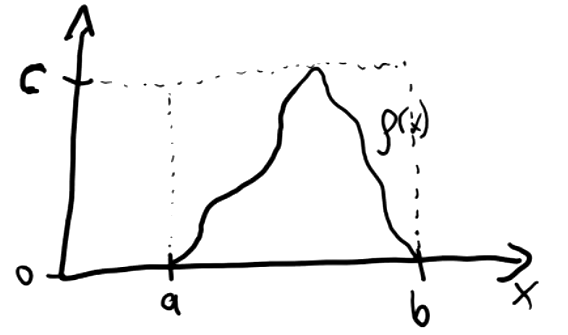
\includegraphics[width=0.4\textwidth]{av-methode}
\end{wrapfigure}
Die Annahme-Verwerfungs-Methode ist ein geometrischer Ansatz, der zufällig
Punkte in einem rechteckigen Bereich generiert, der die
\link{def:dichte}{Dichtefunktion} der gewünschten Verteilung einrahmt.
Notwendige Voraussetzung dafür ist, dass ein endlich großes, die Dichtefunktion
umgebendes Rechteck gefunden werden kann.

Die zufälligen Punkte werden durch skalierte, gleichverteilte Zufallszahlen
bestimmt. Liegt der Punkt unterhalb des Graphs der Dichtefunktion, wird der
X-Wert des Punkts ausgegeben. Damit entspricht die Wahrscheinlichkeit, dass ein
bestimmter Wert als Zufallszahl ausgegeben wird, genau dem Wert der
Wahrscheinlichkeitsdichte an diesem Punkt.

Der folgende Algorithmus gibt eine Folge von Zufallszahlen in der gewünschten
Verteilung aus:

\begin{algorithm}[h!]
\DontPrintSemicolon
\LinesNumbered

\While{1}{
  Erzeuge $x\sim U(a,b)$\;
  Erzeuge $y\sim U(0,1)$\;
  \If{$y\cdot c \le \rho(x)$}{
    gib $x$ aus\;
  }
}


\caption{Annahme-Verwerfungs-Methode}\label{algo:av-methode}
\end{algorithm}

\subsection{Importance-Sampling}

Die Annahme-Verwerfungs-Methode funktioniert dann besonders gut, wenn die Fläche
unter der Dichtefunktion im Vergleich zum einhüllenden Rechteck möglichst gering
ist. In diesem Fall liegen nur wenige Punkte oberhalb der Dichte und müssen
verworfen werden. Ist das einhüllende Rechteck im Vergleich jedoch sehr groß,
beispielsweise weil die Wahrscheinlichkeitsdichte sehr ungleich verteilt ist,
werden viele Punkte verworfen, sodass mehr Zeit für die Erzeugung einer festen
Anzahl an Zufallszahlen erforderlich ist.

Beim Importance-Sampling wird statt eines einhüllenden Rechtecks eine einhüllende
Funktion $h(x)$ verwendet, die weniger Platz als das Rechteck "`verschwendet"'.
Dafür ersetzen wir in Algorithmus \ref{algo:av-methode} die obere Schranke $c$
durch den Wert der Einhüllenden $h(x)$.

Da die Einhüllende $h(x)$ jedoch im Allgmeinen nicht konstant ist, müssen wir
diese Verzerrung korrigieren. Dafür generieren wir die x-Werte der zufälligen
Punkte in der Verteilung der Einhüllenden. Die Einhüllende $h(x)$ besitzt
folgende \link{def:dichte}{Dichte}:
\[H(z) = \frac{1}{\gamma}\cdot\int_a^z h(x) \mathrm{d}x\]
Die Konstante $\gamma = \int_a^b h(x)\mathrm{d}x$ stellt die Normiertheit sicher.

Durch die Inverse $H^{-1}$ der Verteilungsfunktion können mit der
\link{satz:inversionsm}{Inversionsmethode} der Einhüllenden entsprechend
verteilte Zufallszahlen erzeugt werden (da $h(x)$ frei gewählt werden kann, ist
das Invertieren in der Regel kein Problem).

Der entsprechende Algorithmus sieht dann so aus:

\begin{algorithm}[h!]
\DontPrintSemicolon
\LinesNumbered

\While{1}{
  Erzeuge $u\sim U(a,b)$\;
  Setze $x = H^{-1}(u)$\;
  Erzeuge $y\sim U(0,1)$\;
  \If{$y\cdot h(x) \le \rho(x)$}{
    gib $x$ aus\;
  }
}

\caption{Annahme-Verwerfungs-Methode mit Importance Sampling}\label{algo:av-methode-is}
\end{algorithm}

\section{Box-Müller-Polarmethode}

TODO

\end{document}
